\section{\thesection.~Understanding Chord Distributions}

% \againframe<5-6>{disciplines}

\begin{frame}{\insertsectionhead}
  \begin{enumerate}[\color{epflred}1.]
    \item<1-> \textbf{Corpus creation}\\ \citet{Neuwirth2018}.~\citetitle{Neuwirth2018}.
    \item<2-> \textbf{Corpus analysis}\\\citet{Moss2019b}.~\citetitle{Moss2019b}.
    \item<3-> \textbf{Corpus expansion}\\ \citet{Moss2019a}.~\citetitle{Moss2019a} (Diss.).
    % \item \emph{Distant Listening} project (2020--2024)
    % \item Mozart Sonatas (in preparation)
    % \item 24 other composers in preparation (16th--20th c.)
  \end{enumerate}
\end{frame}

\begin{frame}{\insertsectionhead}
  19th-century corpora (9 composers, 289 pieces)
  \begin{columns}
    \begin{column}{.4\linewidth}
      \begin{itemize}
        \item Beethoven: String quartets
        \item Schubert: \emph{Winterreise}
        \item Chopin: Mazurkas
        \item Liszt: \emph{Années de pèlerinage}
        \item Dvorák: \emph{Silhouettes}
        \item Grieg: \emph{Lyrical pieces}
        \item Tchaikovsky: \emph{Seasons}
        \item Debussy: \emph{Suite bergamasque}
        \item Medtner: \emph{Fairy tales}
      \end{itemize}
    \end{column}
    \pause
    \begin{column}{.6\linewidth}
      \begin{figure}
        \centering
        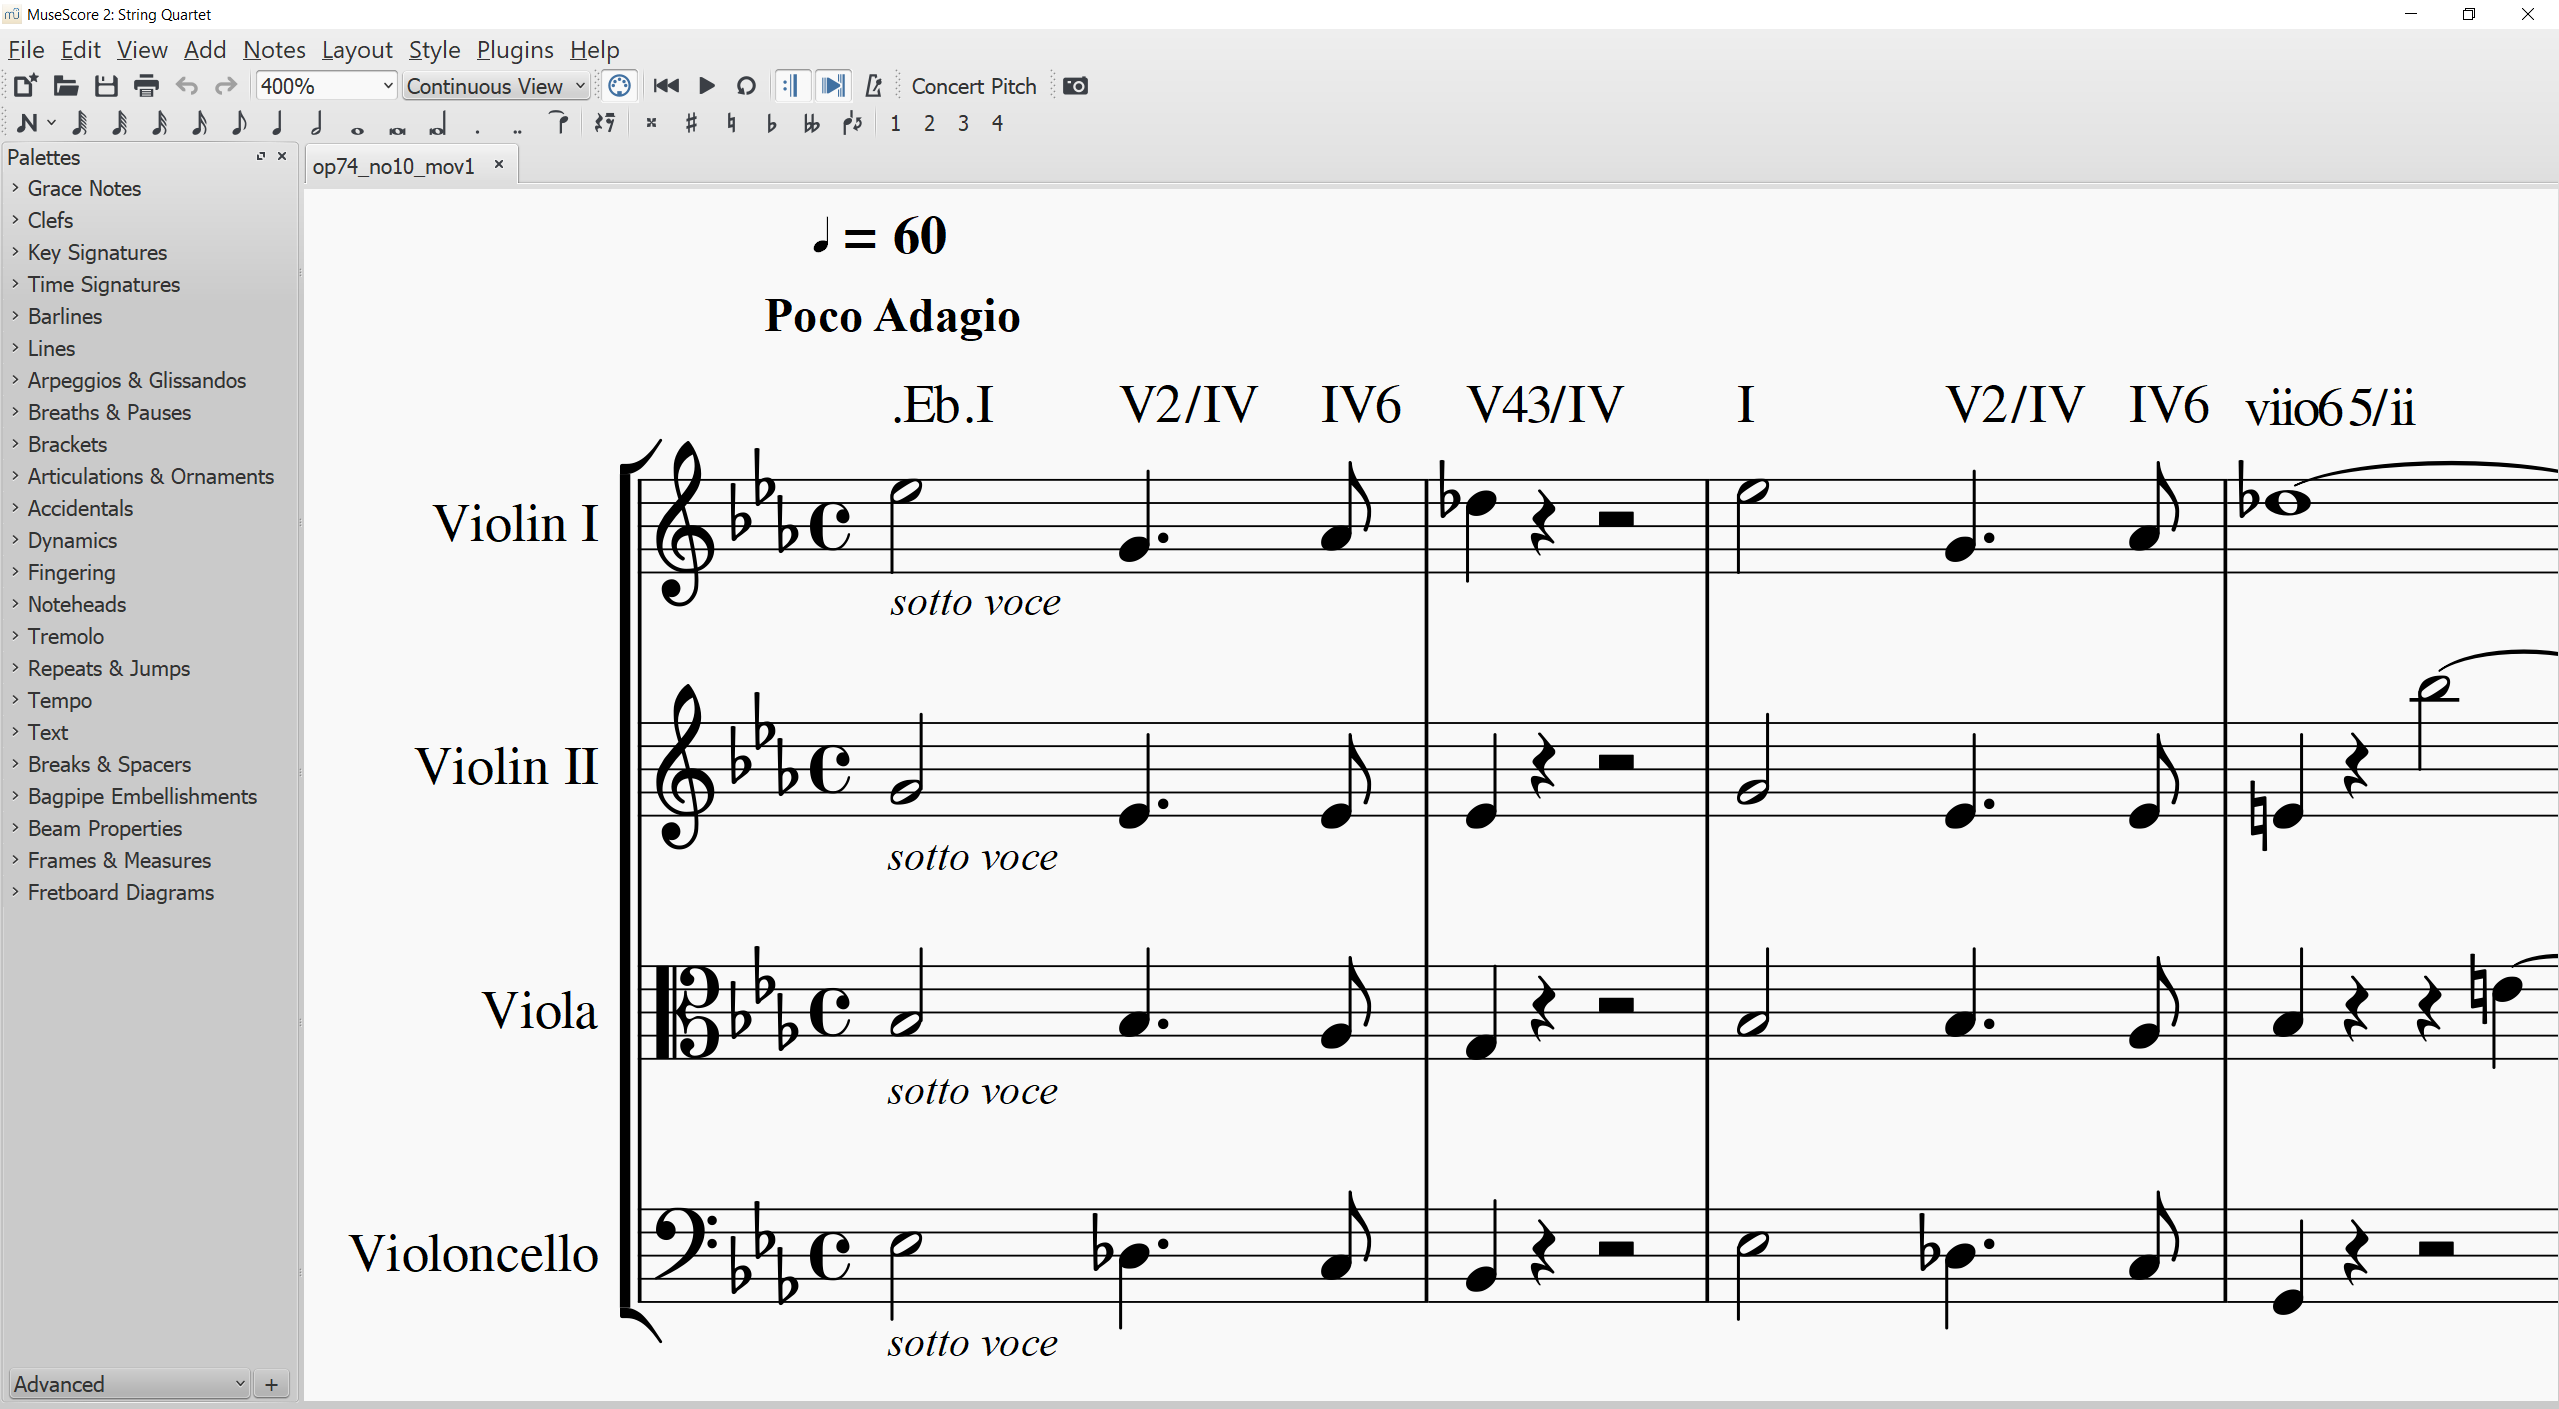
\includegraphics[width=\textwidth,height=.8\textheight,keepaspectratio]{img/musescore_screenshot.png}
        \caption{Chord annotation via \emph{MuseScore}.}
        \label{}
      \end{figure}
    \end{column}
  \end{columns}


\end{frame}

\begin{frame}<1-7>[label=corpus_pipeline]{\insertsectionhead}
  \onslide<1->{The corpus research pipeline}

  \resizebox{\textwidth}{!}{
  \centering
  \tikzstyle{my_arrow} = [->,>=stealth,shorten >= .5em, shorten <= .5em, line width=2pt]
  \begin{tikzpicture}
    \draw [visible on=<2->] (0,0) node (score) {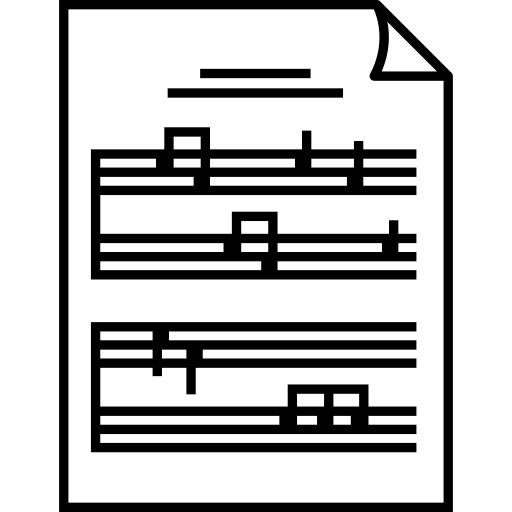
\includegraphics[height=1.5cm]{img/score.png}};

    \draw [visible on=<3->] (3,0) node (file) {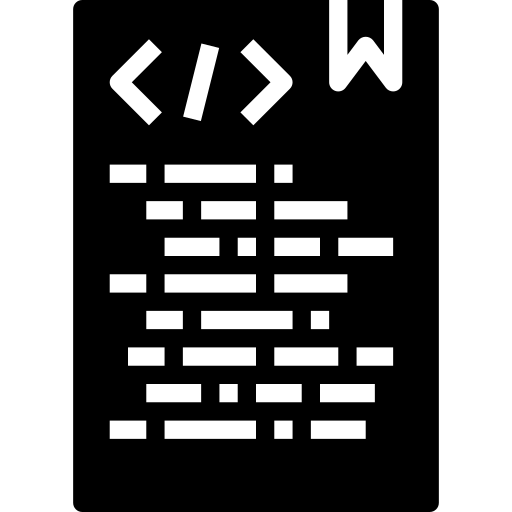
\includegraphics[height=1.5cm]{img/xml.png}};
    \draw [my_arrow,visible on=<3->] (score) -- (file) node [above,midway] {encoding};

    \draw [visible on=<4->] (6.5,3) node (expert) {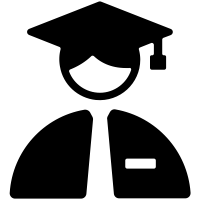
\includegraphics[height=1.5cm]{img/expert.png}};
    \draw [my_arrow,epflred,visible on=<4-7>] (expert) -- (file) node [midway,above left] {\color{epfldark}{analysis}};
    \draw [my_arrow,epflred!30,visible on=<8->] (expert) -- (file) node [midway,above left] {\color{epfldark!30}{analysis}};

    \draw [visible on=<5-7>] (7,0) node (vec) {\footnotesize$x=\begin{bmatrix}I\\V7\\ii6\\V7/IV\\\sharp viio\\\vdots\end{bmatrix}$};
    \draw [visible on=<8->] (7,0) node (vec) {\footnotesize$x=\begin{bmatrix}B\flat\\G\\A\\G\\C\sharp\\\vdots\end{bmatrix}$};
    \draw [my_arrow,visible on=<5->] (file) -- (vec) node [above,midway] {extraction};

    \draw [visible on=<6-7>] (12,0) node (dist) {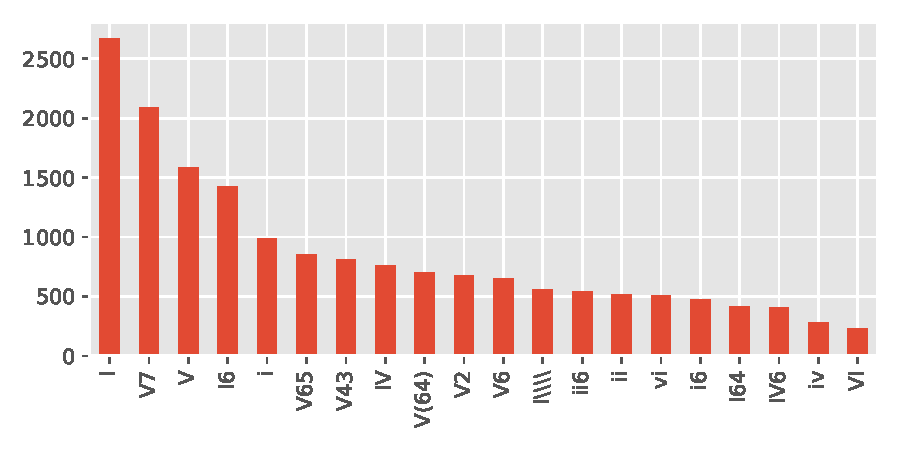
\includegraphics[width=4cm]{img/chord_stats.pdf}};
    \draw [visible on=<8->] (12,0) node (dist) {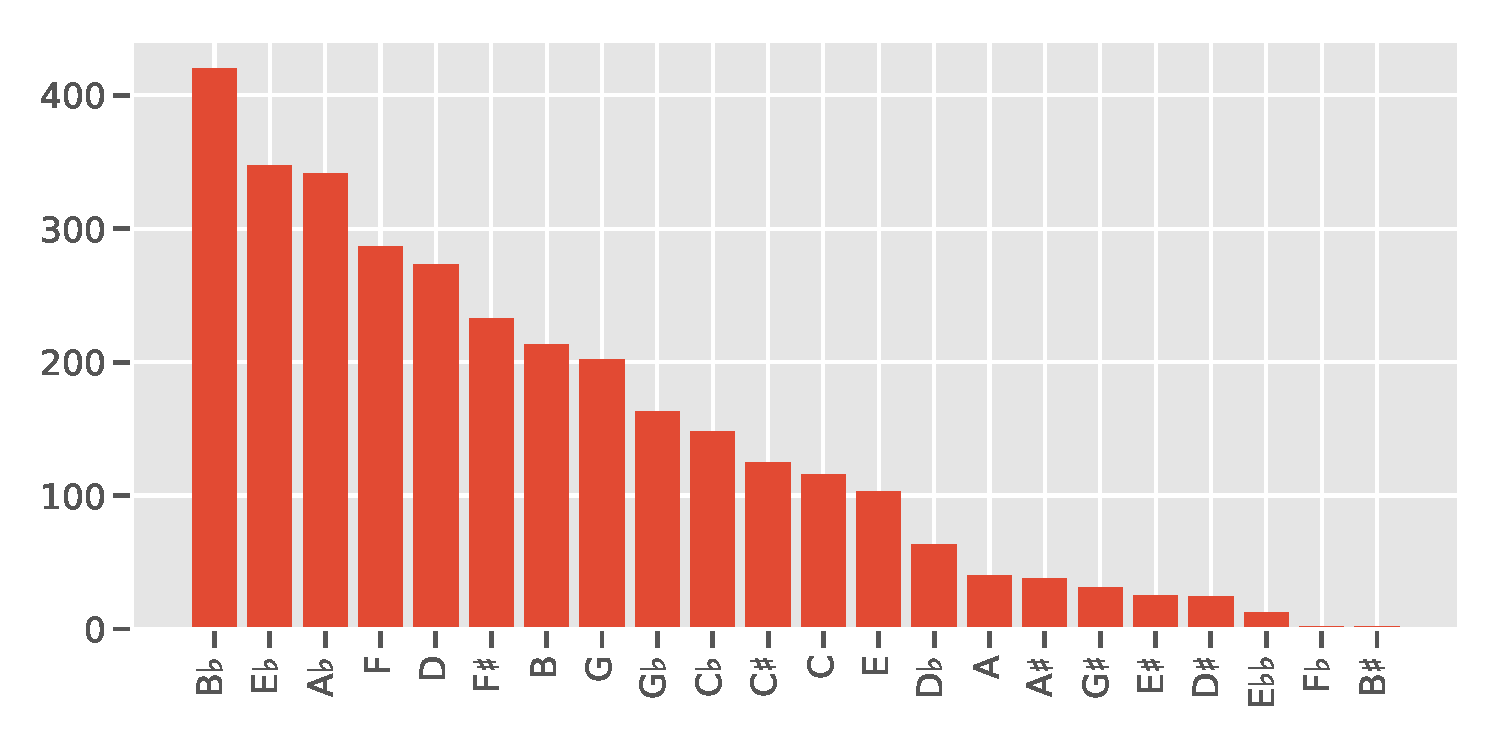
\includegraphics[width=4cm]{img/tpc_dists_sorted.pdf}};
    \draw [my_arrow,visible on=<6->] (vec) -- (dist) node [above, midway] {statistics};

    \draw [my_arrow,visible on=<7->, epflred] (expert) -- (dist) node [above right, midway] {\color{epfldark}{interpretation}};

  \end{tikzpicture}
  }
\end{frame}

\begin{frame}{\insertsectionhead}
  A fundamental distinction in corpus research:

  \begin{itemize}
    \item \alert{all chords} that occur in a corpus $\mathcal C$ (chord tokens), e.g.
  \end{itemize}
  \begin{align*}
    T_{\mathcal C} = \{\, I : 12,\, V7 : 6,\, V : 5,\, ii : 5,\, IV : 4,\, I6 : 2,\, III : 1,\, viio7 : 1\,\}
  \end{align*}
  \pause
  \begin{itemize}
    \item \alert{all unique chords} that occur in a corpus $\mathcal C$ (chord types), e.g.
  \end{itemize}
  \begin{align*}
    t_{\mathcal C} = \{\, I, V7, V, ii, IV, I6, III, viio7 \,\}
  \end{align*}
\end{frame}


\begin{frame}{\insertsectionhead}

  \begin{columns}
    \begin{column}{.7\textwidth}
\def\firstcircle{(0,0) circle (1.2cm)}
\def\secondcircle{(60:2cm) circle (2cm)}
\def\thirdcircle{(120:2cm) circle (1.5cm)}
\tikzstyle{corpus}=[line width=0mm,epflred,fill, opacity=0]
\begin{center}
\begin{tikzpicture}
  \draw[corpus,fill opacity=0.2, visible on=<1->]
    \firstcircle node[black,below,opacity=1] {$\mathcal C_1$};
    %
    \draw[corpus,fill opacity=0.4, visible on=<2->]
    \secondcircle node[black,right,opacity=1] {$\mathcal C_2$};
    %
    \draw[corpus,fill opacity=0.6, visible on=<3->]
    \thirdcircle node[black,left,opacity=1] {$\mathcal C_3$};
    %
    \draw [thick,decorate,decoration={brace,amplitude=10pt},visible on=<4->] (-3,-1.5) -- (-3,4) node [midway, left, xshift=-5mm,align=center]  {Vocabulary:\\3,185 unique chords\\(75,380 chords in total)}; % \\3185 types
    \node [align=center, visible on=<5->] (core) at (3,-1) {Core:\\43 unique chords}; %  $\mathbb C$\\43 types
    \node (intersection) at (-.45,.85) {};
    \draw[->,>=stealth,thick, visible on=<5->] (core) -- (intersection);
\end{tikzpicture}
\end{center}
\end{column}
%
\begin{column}{.3\textwidth}
  \onslide<6->{
\begin{align*}
  \frac{|Core|}{|Vocabulary|} \approx 1.35\text{\%}
\end{align*}}
\end{column}
\end{columns}
\end{frame}

\begin{frame}{\insertsectionhead}
\onslide<1->{
\small
  \begin{align*}
   \text{Core} = \{\;
      & \mathsf{I},\, \mathsf{I6},\, \mathsf{I64},\, \mathsf{i},\, \mathsf{i6},\, \mathsf{i64},\, \nonumber\\
      & \mathsf{ii},\, \mathsf{ii6},\, \mathsf{ii7},\, \mathsf{ii65},\, \mathsf{iio},\, \mathsf{ii\emptyset 7},\, \mathsf{ii\emptyset 43},\, \mathsf{ii\emptyset 2},\, \nonumber\\
      & \mathsf{iii},\, \mathsf{iii6},\, \mathsf{III},\, \nonumber\\
      & \mathsf{IV},\, \mathsf{IV6},\, \mathsf{iv},\, \mathsf{iv64},\, \nonumber\\
      & \mathsf{V},\, \mathsf{V6},\, \mathsf{V64},\, \mathsf{V7},\, \mathsf{V7(4)},\, \mathsf{V65},\, \mathsf{V43},\, \mathsf{V2},\, \nonumber\\
      & \mathsf{vi},\, \mathsf{vi6},\, \mathsf{VI},\, \mathsf{VI6},\, \nonumber\\
      & \mathsf{viio6},\, \mathsf{\sharp viio6},\, \mathsf{\sharp viio43},\, \nonumber\\
      & \mathsf{V65/III},\, \mathsf{V7/IV},\, \mathsf{V2/IV},\, \mathsf{V65/V},\, \mathsf{V43/V},\, \mathsf{V2/V},\, \mathsf{\sharp viio7/vi} \;\}
      \label{eq:core}
  \end{align*}}

  \onslide<2->{
  \normalsize
  Between 45 and 74\% of all chords are core chords!
  }
\end{frame}
%
\note[itemize]{

\item this collection consists of the \alert{typical cases} one would find in a harmony text book
\item consequently, textbook harmonic analysis takes only ~1\% of all chords into account
\item How can this be justified?
}

\begin{frame}{\insertsectionhead}
  $\Rightarrow$ What affects the frequency of chords?
\end{frame}

\begin{frame}{\insertsectionhead}
  \begin{columns}
    \begin{column}{.53\linewidth}
      \textbf{Zipf's law}~\citep{Zipf1949}

      The relation between \alert{frequency}~$f$ and \alert{rank}~$r$ (1st, 2nd,\ldots, $n$th) resembles a power law:
      \begin{align*}
        f(r) \approx \frac{\alpha}{(\beta + r)^\gamma}
      \end{align*}
    \end{column}\hfill
    \pause
    \begin{column}{.47\linewidth}
      \begin{figure}
        \centering
        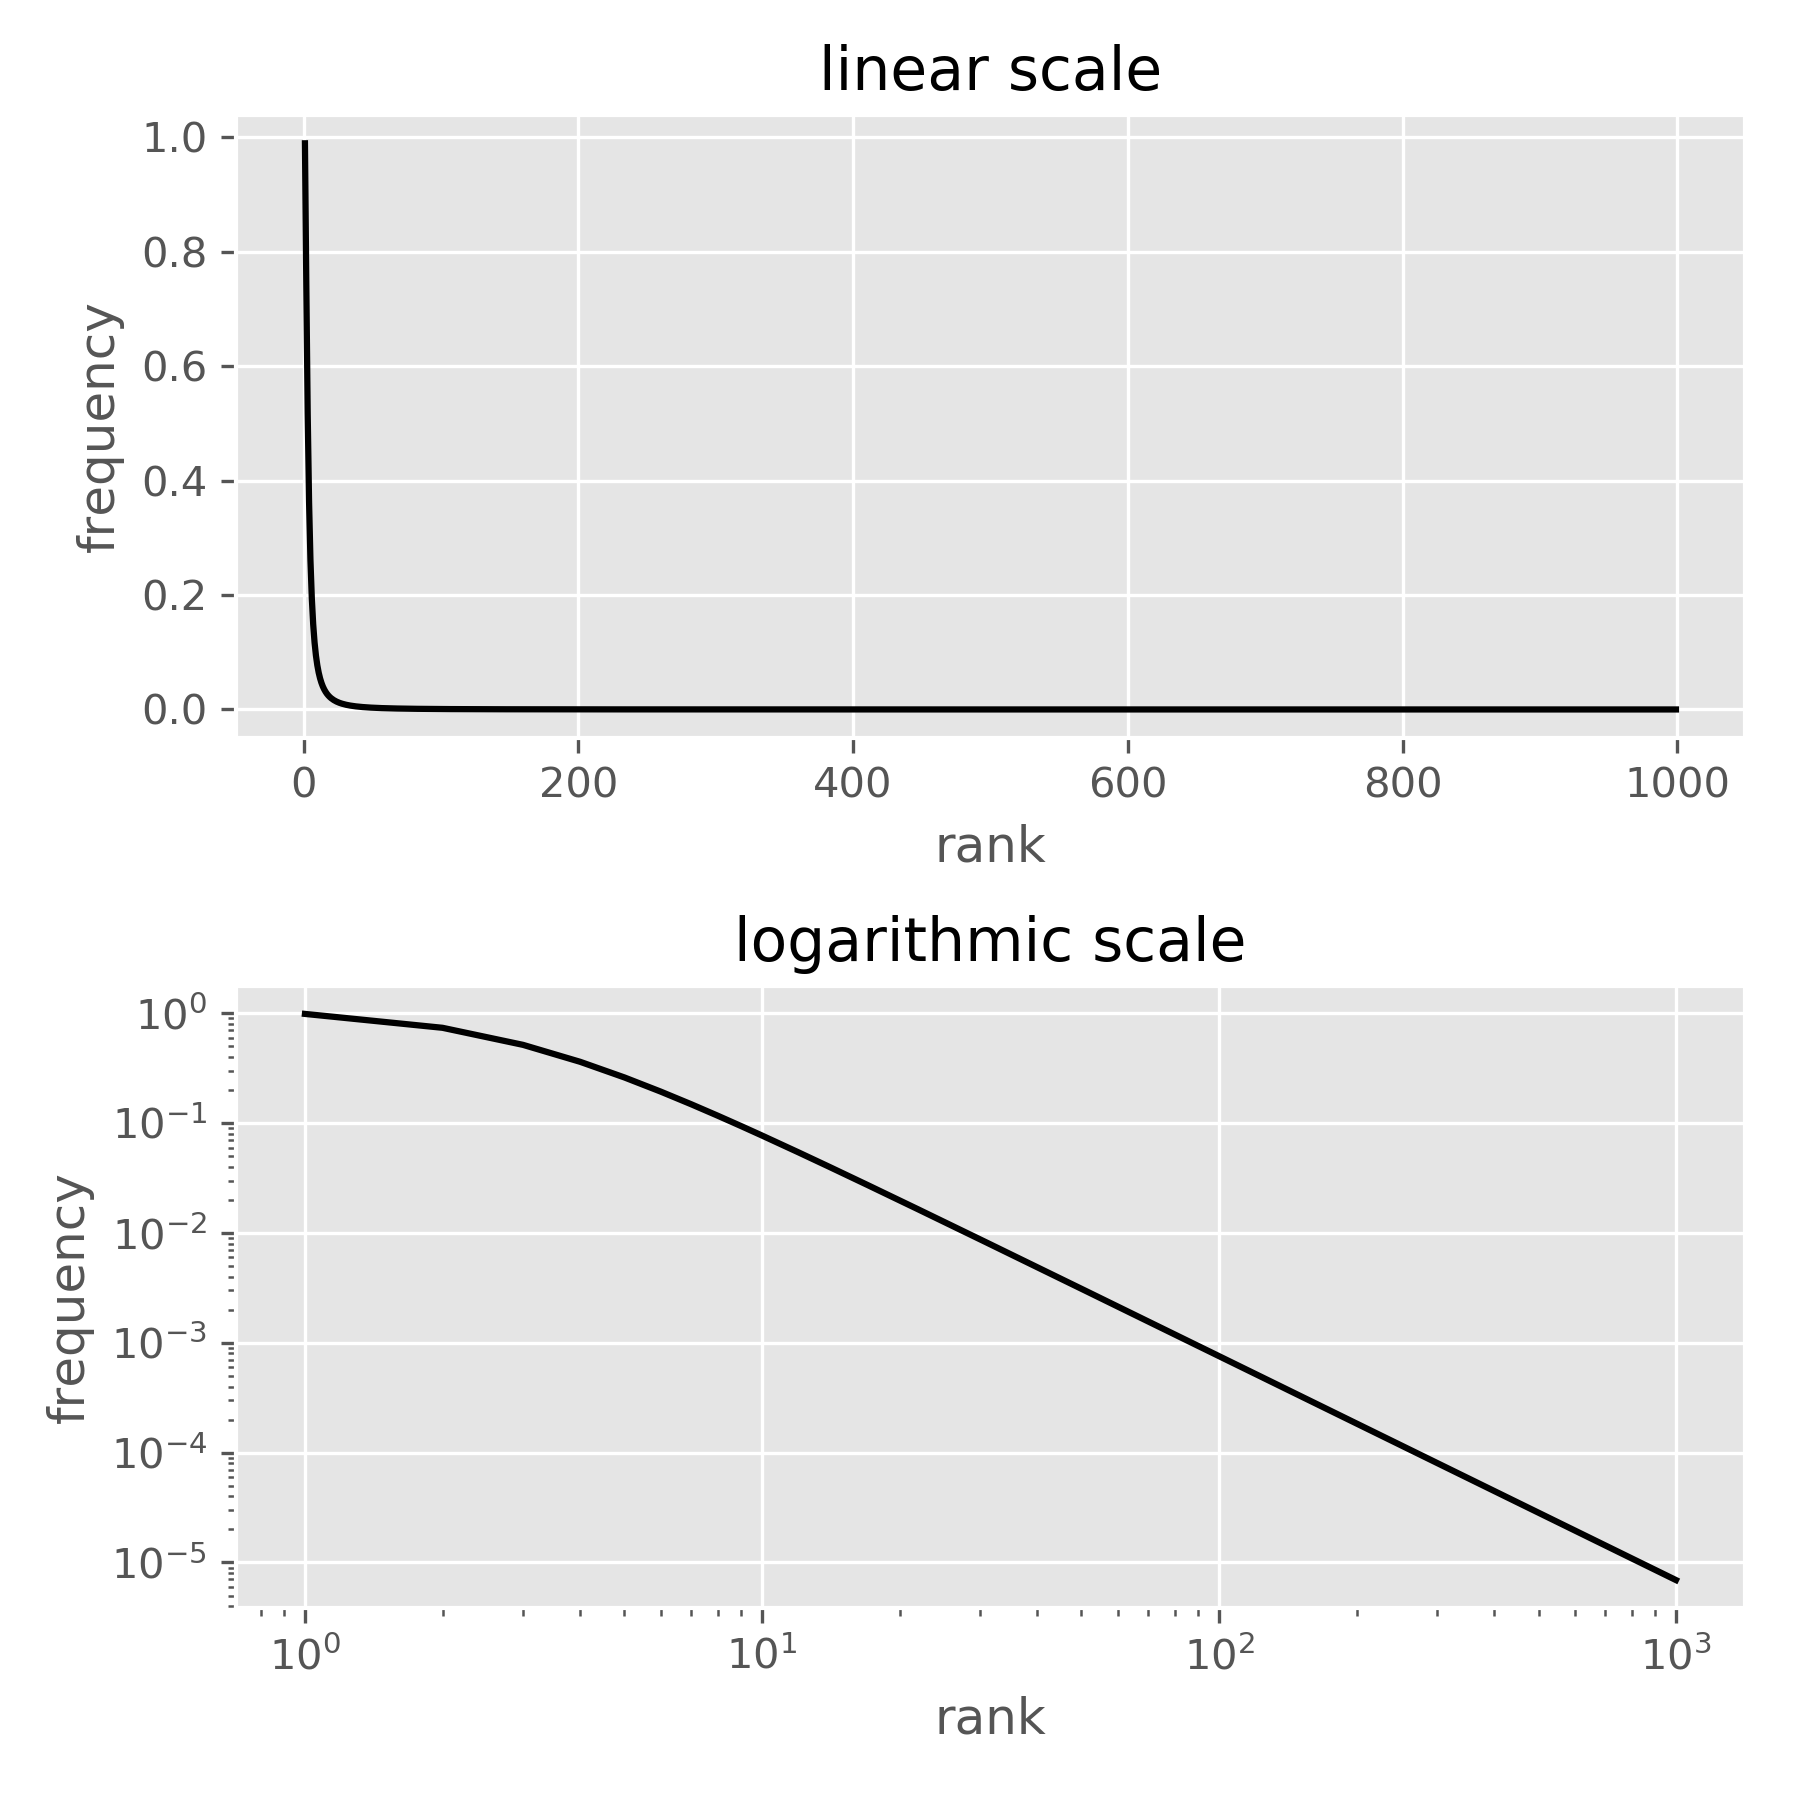
\includegraphics[width=\textwidth]{img/zipf_model.png}
      % \caption{Zipf curve with arbitrary parameters}
      \end{figure}
    \end{column}
  \end{columns}
  % This relation is ubiquitous in linguistics and musicology \parencite{Rohrmeier2008,Piantadosi2014}. Do the annotated corpora \alert{conform} to this phenomenon?
\end{frame}

\begin{frame}{\insertsectionhead}
  \begin{figure}
    % \begin{subfigure}[c]{.6\linewidth}
      \centering
      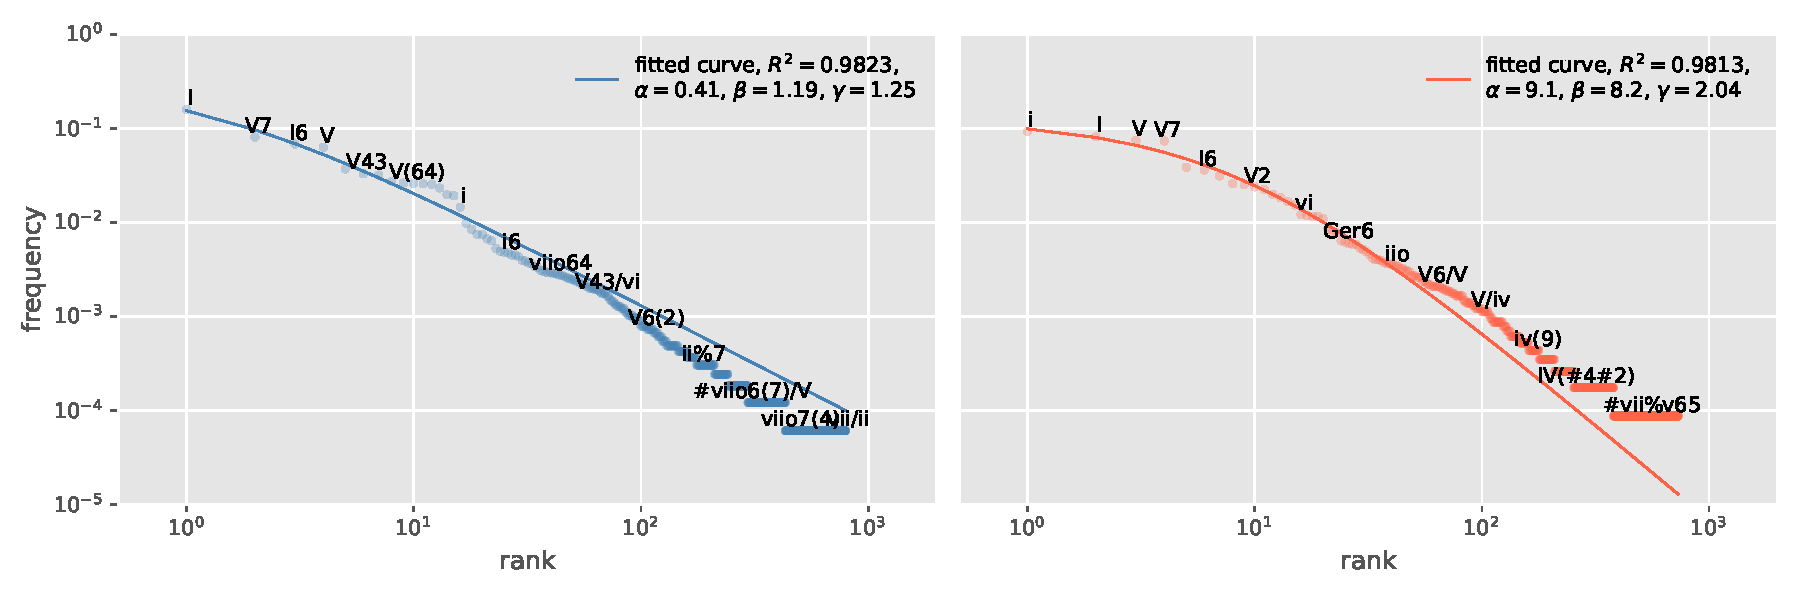
\includegraphics[width=\textwidth]{img/ABC_zipf_mandelbrot.pdf}
      \caption{Chord distribution in Beethoven's string quartets.}
    % \end{subfigure}\vfill
    % \begin{subfigure}[c]{.6\linewidth}
    %   \centering
    %   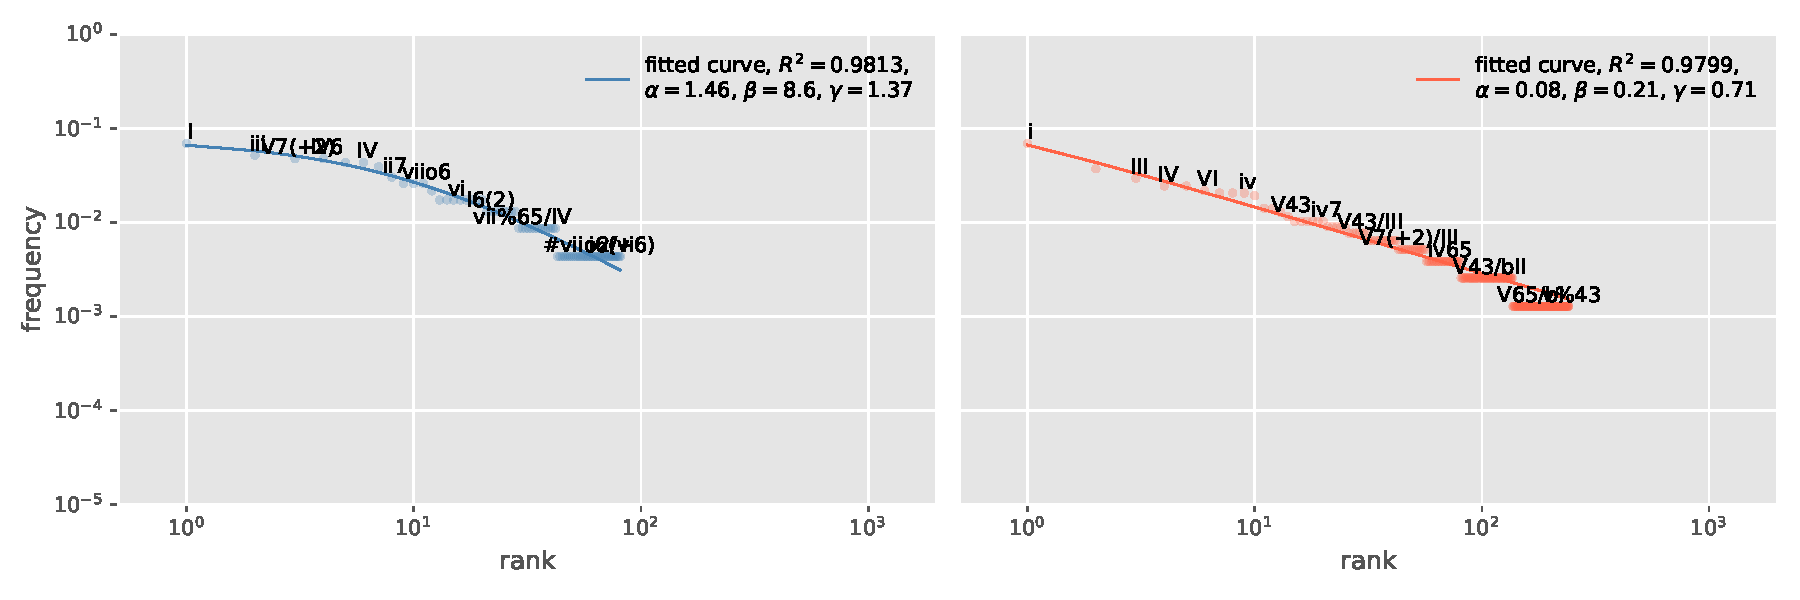
\includegraphics[width=\textwidth]{img/debussy_zipf_mandelbrot.pdf}
    %   \caption{Debussy's \emph{Suite bergamasque}.}
    % \end{subfigure}
  \end{figure}
\end{frame}

\begin{frame}{\insertsectionhead}
  \begin{enumerate}[\color{epflred}1.]
    \item<1-> Zipf's law is found in many domains (e.g. language, social networks, citations, \ldots)
    \item<2-> What is specific about tonal music?
    \item<3-> Many processes could explain this finding~\citep{Piantadosi2014}
    % \item<4-> More sophisticated models are needed
  \end{enumerate}
  \onslide<4->{$\Rightarrow$ Addressing these issues by closer inspecting \alert{deviations} from the model}
\end{frame}

\begin{frame}{\insertsectionhead}
  \begin{figure}
    \centering
    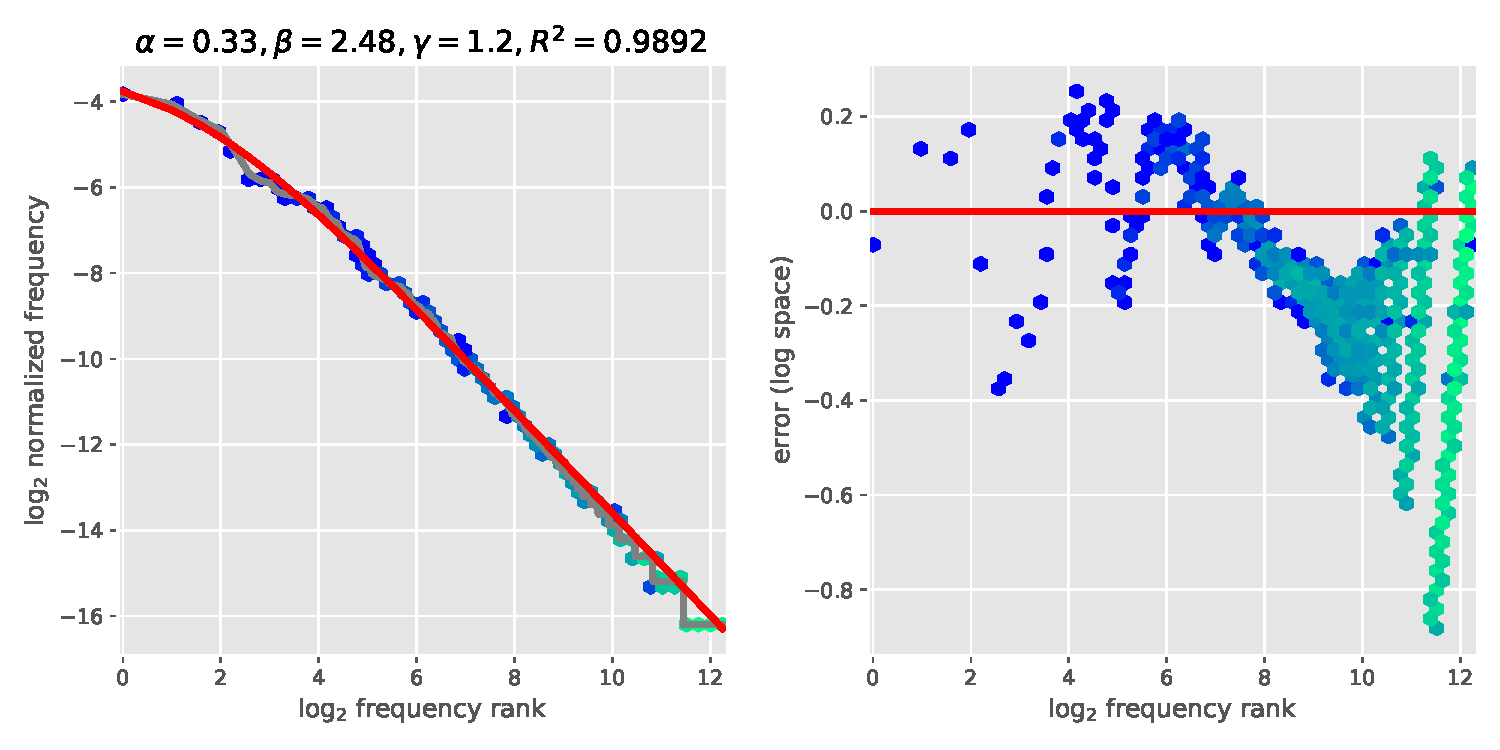
\includegraphics[width=.8\textwidth]{img/freqrank_disterror.pdf}
    \caption{Zipf-fit of chord distribution (left). Deviations from model (right).}
    \label{}
  \end{figure}
\end{frame}

\begin{frame}{\insertsectionhead}
  \begin{itemize}
    \item<1-> \alert{new insight}: systematic deviations from standard models of chord distributions
    \item<2-> development of more advanced models in future research
    \item<3-> impossible without the computational approach
  \end{itemize}

\end{frame}

% \begin{frame}{Summary and Prospects}
%   \begin{enumerate}[\color{epflred}1.]
%     \item \ldots
%     \item \ldots
%     \item \ldots
%     \label{}
%   \end{enumerate}
% \end{frame}
